Ein wichtiger Aspekt dieser Bachelorarbeit ist es, den Studierenden den Einstieg in die Kanalkodierung mit diesem Paket zu erleichtern. Um das Verständnis der Verfahren zu verbessern, wurden Visualisierungen geschaffen, die den Ablauf der Kodierung und Dekodierung genauestens darstellen.

Um die Visualisierungen zu erhalten, gibt es in jeder Funktion einen Parameter (\texttt{visualize}) der mit \texttt{TRUE} gesetzt werden muss, um die Visualisierung zu erhalten. Alle Beispiele in den nächsten Kapitel werden mit Punktierung durchgeführt, da sich die Visualisierung ohne Punktierung nur ein wenig vereinfachen. Die erzeugten PDF-Dokumente werden mit \emph{RMarkdown} und dem darin enthaltenen \LaTeX - und Ti\textit{k}Z-Code erzeugt. Deswegen ist es auch notwendig, dass der Benutzer des Paketes, \LaTeX\ und die wichtigsten Erweiterungen dazu installiert hat.

Da eine lehrreiche Visualisierung nur Sinn mit sehr kurzen Bitfolgen macht, ist die Darstellung auch beschränkt, da ansonsten die Datenflut für den Nutzer nicht mehr bewältigbar wäre. Nebenbei wäre eine visuell schöne Darstellung auch nicht mehr möglich. Deswegen wird ab einer Nachrichtenlänge die größer als 10 ist, eine Warnung ausgegeben. Tatsächlich wird im erzeugten Dokument, ab einer Länge von \textbf{18 Bits}, die Nachrichten abgeschnitten.

Die erzeugten PDF-Dokumente werden im Installationsordner des Paketes abgelegt, der im Programmverzeichnis von R liegt. Dort liegen sie im \textbf{pdf-Ordner}. Mit der Hilfsfunktion \texttt{TurboOpenPDF} lassen sich bereits erzeugte Dokumente nochmals öffnen. Möchte man diese weiterverwenden bietet sich an, die geöffneten Dokumente neu in einem gewünschten Ordner abzuspeichern.

Die Dokumente werden aus reinem \LaTeX -Code erzeugt, dieser ist ebenfalls in dem oben erwähnten Ordner zu finden. Dieser Code kann verwendet werden, um die Grafiken oder Tabellen im Visualisierungsbericht, selbst in einem Dokument nachzustellen.

Zuerst wird in Kapitel~\ref{sec:visualization_punctuationPermutation} die Visualisierung von Permutations- und Punktierungsmatrix vorgestellt. Im Anschluss erfolgen in Kapitel~\ref{sec:visualization_encode} und \ref{sec:visualization_decode} die Erklärung der erzeugten Berichte von Kodierung und Dekodierung. Am Schluss werden noch alle Darstellungen der Simulationen in Kapitel~\ref{sec:visualization_simulation} an einem Beispiel gezeigt. 
\section{Permutationsmatrix und Punktierungsmatrix}
\label{sec:visualization_punctuationPermutation}
Bei der Erzeugung der beiden Matrizen können diese im RStudio dargestellt werden. Das ist vor allem nützlich bei der Permutationsmatrix, da dort erkennbar ist, wie die Matrix von der Initialisierungsmatrix entsteht und daraus der Permutationsvektor abgeleitet wird. 

\begin{lstlisting}[caption=Visualisierung der Permutationsmatrix, label={lst:visualizePermutation}, float=th]
input2 <- c(1,0,1,1,0,1)
permutation.vector.cyclic <- TurboGetPermutation(length(input2), coder, "CYCLIC", list(cols=4, rows=2, distance=2), TRUE)
[1] "Initial-Matrix"
     [,1] [,2] [,3] [,4]
[1,]    0    2    4    6
[2,]    1    3    5    7
[1] "Interleaver-Matrix:  CYCLIC"
     [,1] [,2] [,3] [,4]
[1,]    0    2    4    6
[2,]    5    7    1    3
> permutation.vector.cyclic
[1] 0 5 2 7 4 1 6 3

permutation.vector.helical <- TurboGetPermutation(length(input2), coder, "HELICAL", list(cols=4, rows=2), TRUE)
[1] "Initial-Matrix"
     [,1] [,2] [,3] [,4]
[1,]    0    1    2    3
[2,]    4    5    6    7
[1] "Interleaver-Vector:  HELICAL"
[1] 0 5 2 7 0 5 2 7
\end{lstlisting}

In Listing~\ref{lst:visualizePermutation} wird zuerst der selbe Eingangsvektor erzeugt, der auch in Kapitel~\ref{cha:examples} verwendet wurde. Danach wird ein Permutationsvektor vom Typ \texttt{CYCLIC} erzeugt. Dabei wird zuerst eine Initialisierungsmatrix erstellt, bei der dann die Bits jeder Zeile, um den Index multipliziert mit der Distanz nach rechts verschoben werden. Der Index fängt bei null an zu zählen, also wird die zweite Zeile um $1*2 = 2$ nach rechts verschoben. Die erste Zeile bleibt immer unverändert. Die daraus resultierende Matrix wird dann von oben nach unten spaltenweise ausgelesen, wie im Beispiel zu sehen.

Beim zweiten Beispiel wird ein Permutationsvektor vom Typ texttt{HELICAL} kreiert. Dabei wird nicht die Initialisierungsmatrix verändert, sondern nur die Art der Auslesung des Permutationsvektors ist für diesen Typ entscheidend. Das ist ebenfalls beim Typ texttt{BLOCK} und texttt{DIAGONAL} so. Bei diesem Beispiel werden die Bits von links oben nach rechts unten ausgelesen. Wird dabei das Ende der Matrix erreicht, wir das nächste Bit in der nächsten Spalte von der ersten Zeile ausgelesen. Beim Typ texttt{DIAGONAL} wird vergleichsweise das erste Bit in der selben Spalte als nächstes verwendet.

\begin{lstlisting}[caption=Visualisierung der Punktierungssmatrix, label={lst:visualizePunctuationMatrix}, float=th]
punctuation.matrix <- TurboGetPunctuationMatrix(c(1,1,0,0,1,1), TRUE)
[1] "Punctuation-Matrix:"
     [,1] [,2]
[1,]    1    0
[2,]    1    1
[3,]    0    1
\end{lstlisting}

Zur Verwendung einer Punktierung beim Turbo-Kode-Verfahren benötigt es eine Punktierungsmatrix, diese lässt sich mit einer Hilfsfunktion wie in Listing~\ref{lst:visualizePunctuationMatrix} erzeugen. Bei der Visualisierung handelt es sich um eine einfache Darstellung der resultierenden Matrix. Wichtig dabei ist, dass der mitgegebene Vektor immer durch 3 teilbar sein muss, also hat die Matrix immer drei Zeilen. Bei einer 0 wird das Bit gelöscht und bei einer 1 behalten.

\FloatBarrier
\section{Kodierung}
\label{sec:visualization_encode}
Als erstes werden immer Informationen zum verwendeten Kodierer dargestellt. Diese Darstellung wird allerdings bereits bei der Bachelorarbeit von Martin Nocker über Faltungskodes erklärt und deshalb hier nicht näher angeführt. \cite{nocker}

\begin{figure}[th]
\centering
	\begin{subfigure}{0.45\textwidth}
	\centering
	\fbox{ 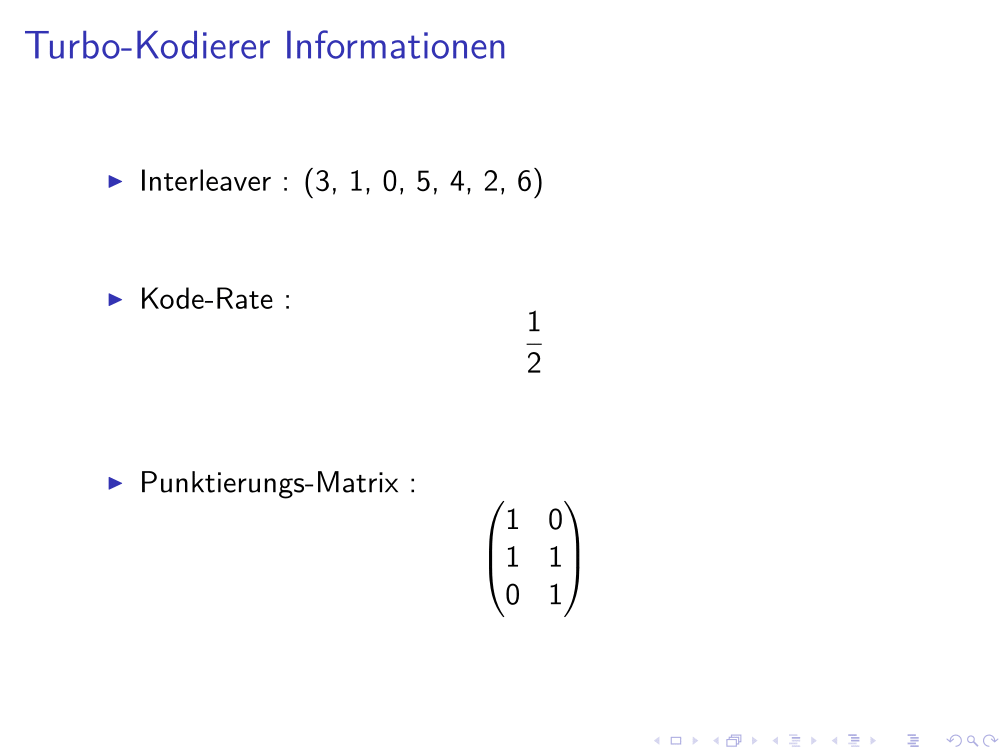
\includegraphics[width=\ScaleIfNeeded]{pictures/TurboEncodePunctured1} }
	\caption{Folie mit Turbo-Kodierer Informationen}
	\label{pic:TurboCoderInformation}
	\end{subfigure}
	\qquad
	\begin{subfigure}{0.45\textwidth}
	\centering
	\fbox{ 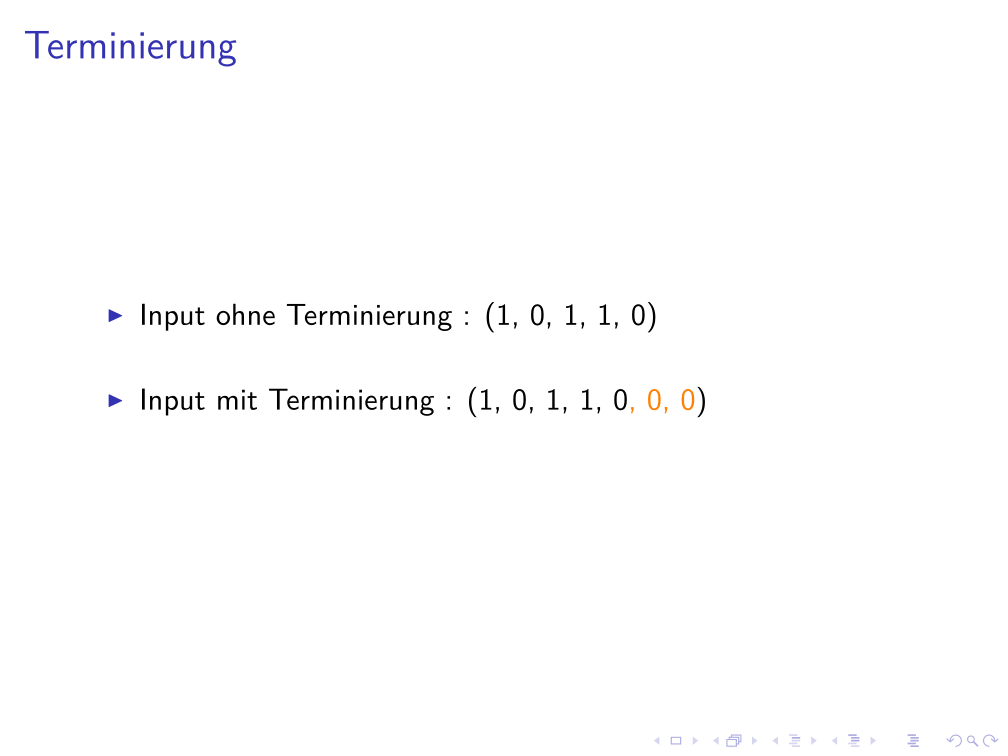
\includegraphics[width=\ScaleIfNeeded]{pictures/TurboEncodePunctured2} }
	\caption{Folie mit Terminierungsdarstellung bei der Kodierung}
	\label{pic:TerminationEncode}
	\end{subfigure} 
\caption{Folien mit allgemeinen Informationen vor der Kodierung}
\label{pic:SlidesCommonEncode}
\end{figure}  

Die genauen Informationen über die Turbo-Kodierer Parameter finden sich auf den nächsten Folien, wie in Abbildung~\ref{pic:TurboCoderInformation} dargestellt. Dort wird als erstes der Permutationsvektor angezeigt, der beim Interleaver verwendet wird. Das stellt die Reihenfolge der Bits dar, wie sie aus dem Interleaver kommen. Als nächstes wird die Koderate angezeigt, die bei einem normalen Turbo-Kodierer ohne Punktierung immer $\frac{1}{3}$ ist. Hier wird der Wert mit Punktierung berechnet und dargestellt. Am Ende wird noch die Punktierungsmatrix abgebildet. 

In Abbildung~\ref{pic:TerminationEncode} sieht man die Darstellung der Terminierung. Da die Faltungskodierer eine Terminierung vorsehen, müssen bei der Eingangsbitfolge noch die Terminierungsbits berechnet werden, damit der Kodierer am Ende im Ausgangszustand ist. Diese Bits werden an die Ausgangsnachricht angefügt und in Orange dargestellt. Bei einem nicht rekursiven Faltungskodierer sind es immer 0er, jedoch bei einem rekursiven müssen sie berechnet werden.

\begin{figure}[th]
\centering
\fbox{ 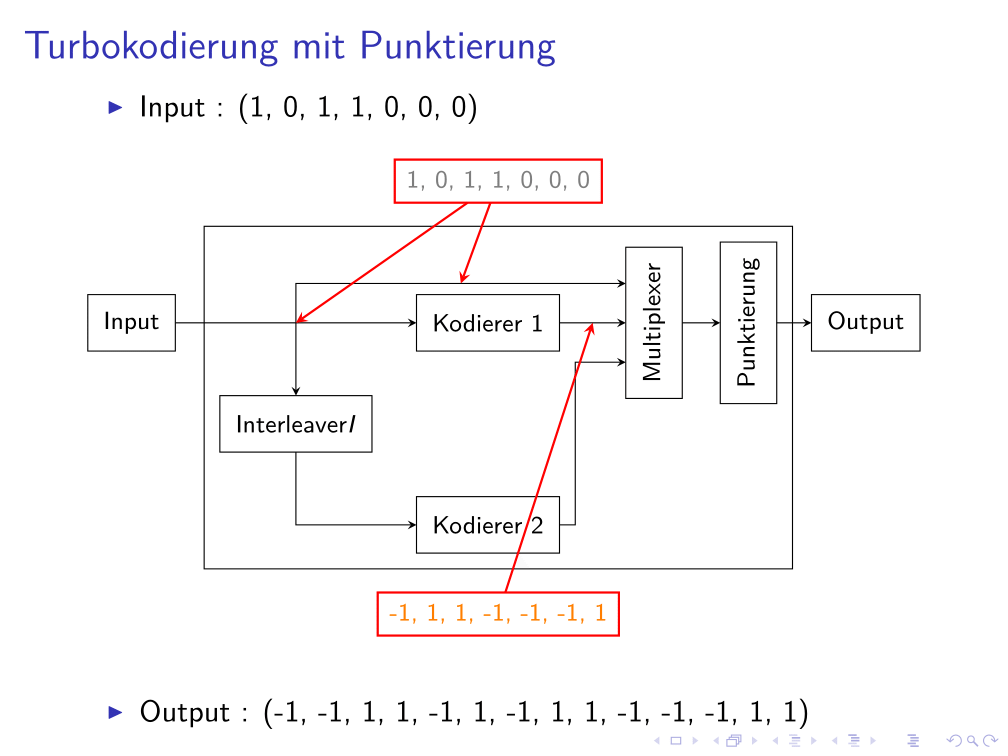
\includegraphics[width=\ScaleIfNeeded]{pictures/TurboEncodePunctured3} }
\caption{Folie der Turbo-Kode Schaltung}
\label{pic:TurboEncode}
\end{figure}
	
\begin{figure}[th]
\centering
\fbox{ 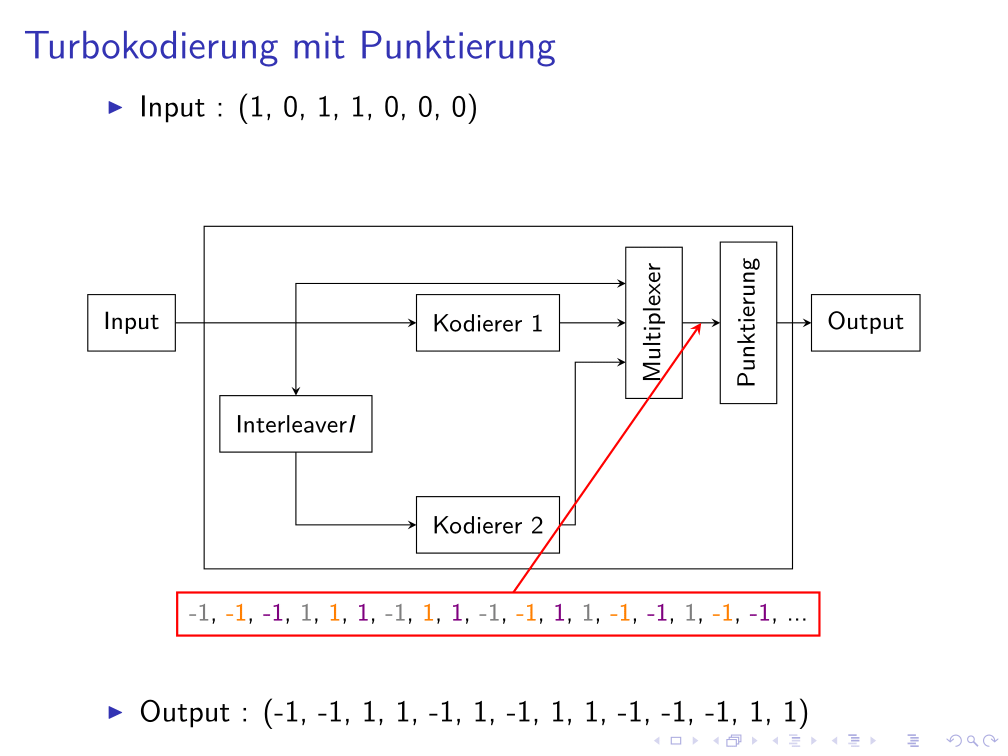
\includegraphics[width=\ScaleIfNeeded]{pictures/TurboEncodePunctured4} }
\caption{Folie mit Ergebnis des Multiplexers}
\label{pic:TurboEncodeMultiplexer}
\end{figure}  

Auf der nächsten Folie, die in Abbildung~\ref{pic:TurboEncode} dargestellt ist, ist die komplette Schaltung abgebildet, die für die Kodierung nötig ist. Die beiden Kodierer sind die übergebenen Faltungskodierer, die verwendet werden, um einen Teil des resultierenden Signals zu erhalten. Die Bits sind eingefärbt, damit man das Ergebnis nach dem Multiplexer, aus den Farben folgern kann. Die drei Einzelbitfolgen werden so ineinander verschachtelt, damit jeweils ein Bit aus Teilfolge eins, zwei und drei hintereinander sind. Das lässt sich am Besten mit Abbildung~\ref{pic:TurboEncodeMultiplexer} zeigen. Dort sieht man sehr leicht, wie der Multiplexer die Bitfolgen ausgibt. Der Interleaver ($I$) permutiert das Signal, damit die Distanz zwischen zwei Kodewörtern erhöht wird.

\begin{figure}[th]
\centering
\fbox{ 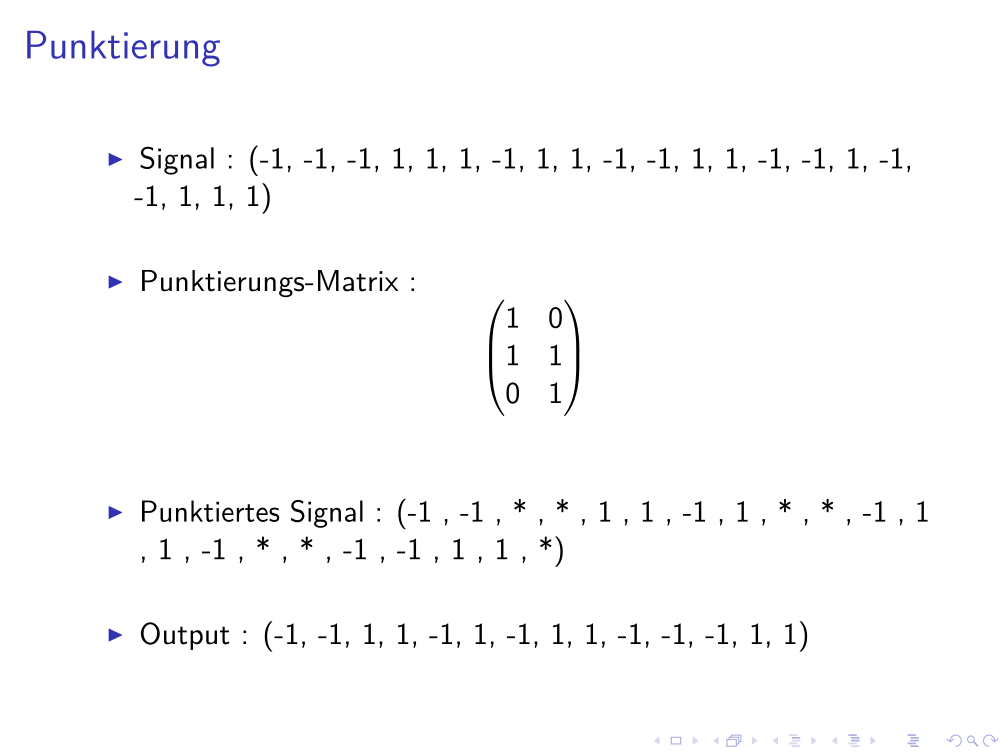
\includegraphics[width=\ScaleIfNeeded]{pictures/TurboEncodePunctured5} }
\caption{Folie mit Darstellung der Punktierung}
\label{pic:TurboEncodePuncturing}
\end{figure}  

Auf der letzten Abbildung~\ref{pic:TurboEncodePuncturing} ist die Punktierung sehr einfach dargestellt. Dabei wird jedes zu löschende Bit mit einem Stern * angezeigt. Somit lässt sich einfach nachvollziehen, dass die Bitfolge von oben nach unten spaltenweise durch die Punktierungsmatrix geführt wird und bei einer 0 dieses Bit entfernt wird. Am Ende ist das fertige Signal dargestellt, das dann auf den Übertragungskanal gelangt. 

Bei der Kodierung ohne Punktierung ist der Ablauf exakt der Selbe, nur wird eben das Signal am Ende nicht punktiert, sondern direkt ausgegeben.

\FloatBarrier
\section{Dekodierung}
\label{sec:visualization_decode}
Bei der Dekodierung werden wieder zuerst die Faltungskodierer Informationen angezeigt und im Anschluss noch die Turbo-Dekodierer Informationen. Da dies jedoch in Kapitel~\ref{sec:visualization_encode} bereits gezeigt wurde, wird das jetzt nicht noch einmal wiederholt. Nachdem die Visualisierung in diesen Kapiteln alle mit Punktierung vorgestellt werden, muss zuerst bei der Dekodierung die punktierten Bits wieder eingefügt werden.

\begin{figure}[th]
\centering
\fbox{ 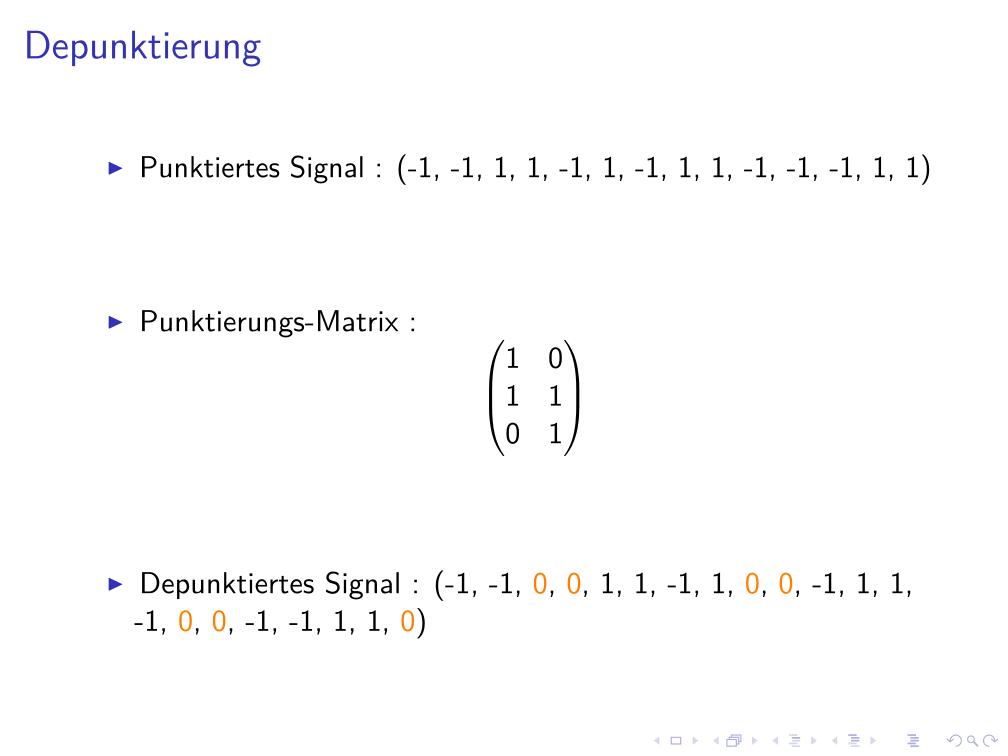
\includegraphics[width=\ScaleIfNeeded]{pictures/TurboDecodePunctured1} }
\caption{Folie zur Veranschaulichung der Depunktierung}
\label{pic:TurboDecodeDepuncturing}
\end{figure}

Wie in Abbildung~\ref{pic:TurboDecodeDepuncturing} zu sehen ist, wird an den 0er Stellen der Punktierungsmatrix, wieder eine 0 in das Eingangssignal eingefügt. Diese Bits sind in Orange eingefärbt. Da eine 0 weder eine -1 noch eine +1 bevorzugt, also beide Signalpegel gleich wahrscheinlich sind, wird dieses Bit eingefügt. Dieses Vorgehen ist nur mit einem Soft-Dekodierer möglich, da dieser sämtliche Signalpegel auswertet. 

\begin{figure}[th]
\centering
\fbox{ 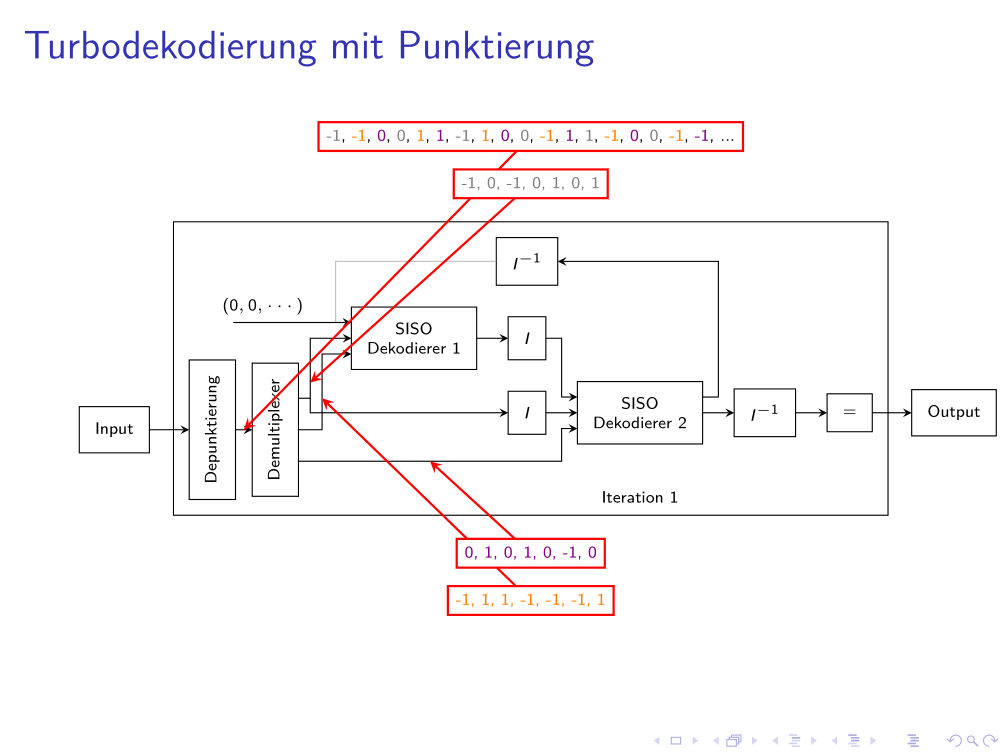
\includegraphics[width=\ScaleIfNeeded]{pictures/TurboDecodePunctured2} }
\caption{Folie der Turbo-Dekode Schaltung}
\label{pic:TurboDecode}
\end{figure}

Auf der nächsten Folie ist, wie in Abbildung~\ref{pic:TurboDecode} zu sehen, die Dekodierer-Schaltung von Turbo-Kodes zu sehen. Dabei wird das Eingangssignal am Anfang depunktiert und danach in den Demultiplexer geschickt, der das Signal wieder in drei Teile aufspaltet. Dabei sind wieder die Bits farblich markiert, damit leicht zu sehen ist, wie das Demultiplexing funktioniert.

\begin{figure}[th]
\centering
\fbox{ 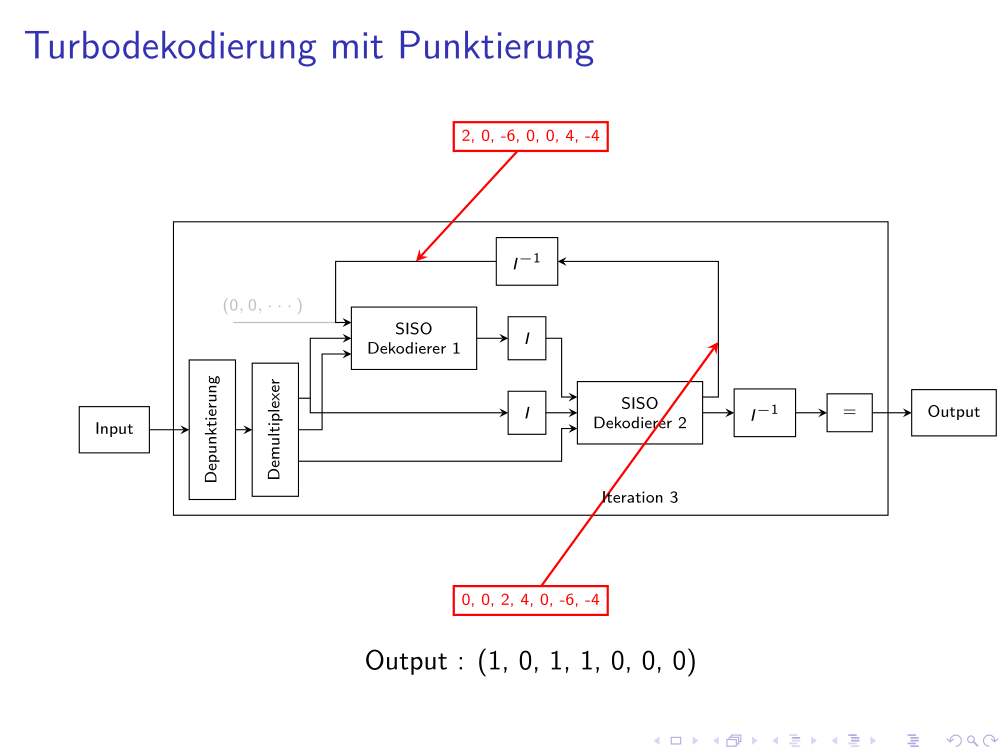
\includegraphics[width=\ScaleIfNeeded]{pictures/TurboDecodePunctured3} }
\caption{Folie zur Darstellung der Turbo-Dekode Rückführung}
\label{pic:TurboDecodeBack}
\end{figure}

Nachdem die beiden Soft-Dekodierer durchlaufen sind, wird das Ergebnis des zweiten Dekodierers wieder zurückgeführt, auf den Eingang des ersten Dekodierers, wie in Abbildung~\ref{pic:TurboDecodeBack}. Je nach Anzahl von mitgegebenen Iterationen, wird so das Ergebnis mehrmals zurückgeführt. Die Interleaver ($I$) und Deinterleaver ($I^{-1}$) permutieren das Signal mit dem miteglieferten Permutationsvektor, damit in die Dekodierer immer die selbe Bitreihenfolge geschickt wird. Am unteren Rand der Folie ist immer die aktuelle Ausgangsbitfolge zu sehen, die aktuell Zustande kommen würde. Damit ist gut zu sehen, wenn sich durch mehrere Iterationen das Ergebnis ändert.

\begin{figure}[th]
\centering
	\begin{subfigure}{0.45\textwidth}
	\centering	
	\fbox{ 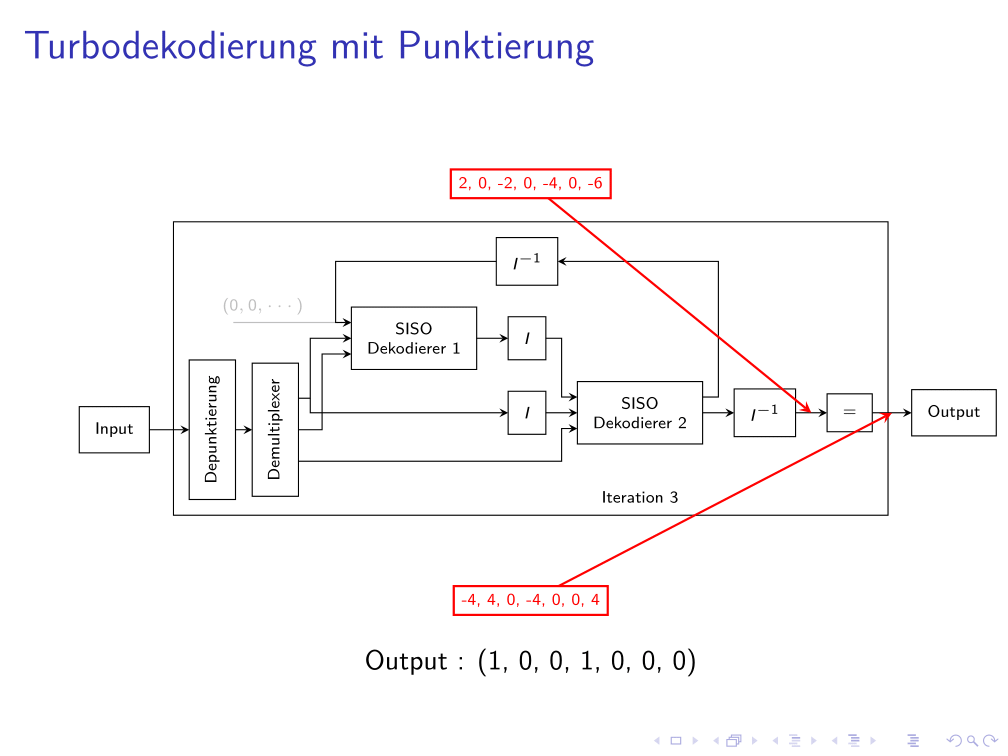
\includegraphics[width=\ScaleIfNeeded]{pictures/TurboDecodePunctured4} }
	\caption{Folie zur Berechnung der Ausgangsbitfolge}
	\label{pic:TurboDecodeResult}
	\end{subfigure}
	\qquad
	\begin{subfigure}{0.45\textwidth}
	\centering
	\fbox{ 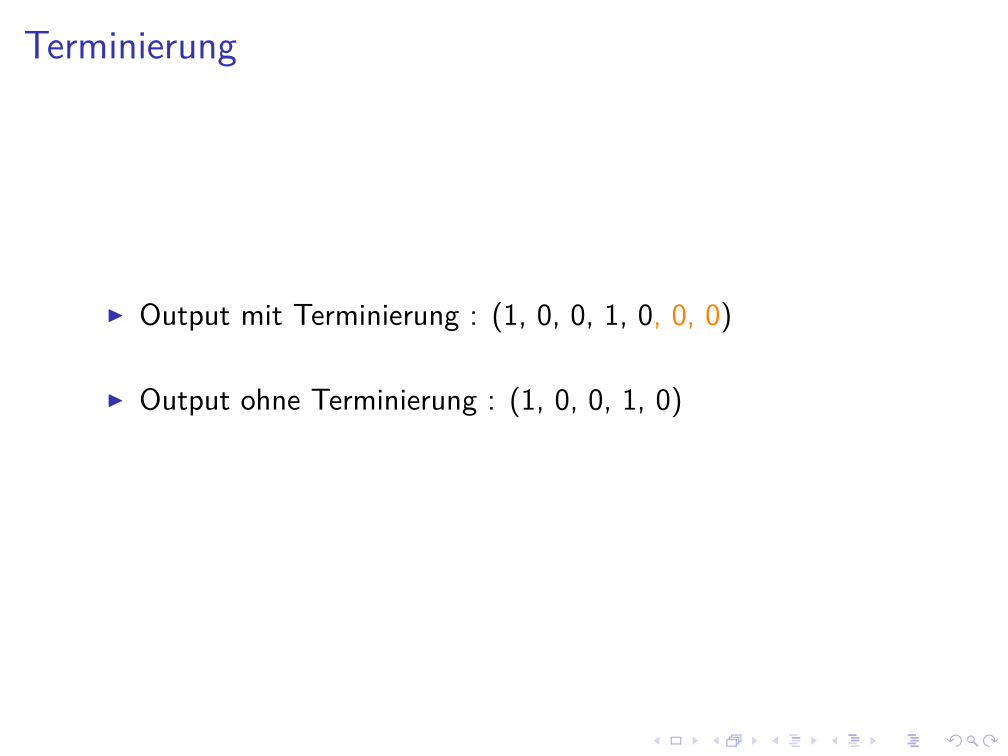
\includegraphics[width=\ScaleIfNeeded]{pictures/TurboDecodePunctured5} }
	\caption{Folie zur Entfernung der Terminierungsbits}
	\label{pic:TurboDecodeTerminate}
	\end{subfigure}
\caption{Folien zur Finalisierung der Dekodierung}
\end{figure}

Nachdem alle Iterationen abgeschlossen sind, wird das Ausgangssignal des zweiten Dekodierers noch einmal permutiert und dann erfolgt die schlussendliche Berechnung, die zur Ausgangsbitfolge führt, wie in der Abbildung~\ref{pic:TurboDecodeResult} zu sehen. Dabei kommt einen Formel zu tragen, die in Kapitel~\ref{sec:parallelConvCodes} nachzulesen ist. Dabei wird die Originalnachricht zusammen mit den beiden Ergebnisse der Dekodierer verwendet. Da bei der Ausgangsbitfolge noch die Terminierungsbits inkludiert sind, werden diese noch in der Abbildung~\ref{pic:TurboDecodeTerminate} entfernt. Dabei werden die eingefärbten Bits entfernt und man erhält die dekodierte Ausgangsbitfolge.

\FloatBarrier
\section{Simulationen}
\label{sec:visualization_simulation}
Auch bei den Simulationen stehen Visualisierungsberichte zur Verfügung, die das Resultat der Simulation sehr einfach und verständlich darstellen. Dabei werden am Anfang immer Informationen zum Kodierer gezeigt, die wir jedoch schon aus Kapitel~\ref{sec:visualization_encode} kennen und deswegen nicht mehr erklärt werden. Danach folgen Informationen zu den Simulationsparametern und am Ende noch eine Grafik mit den Ergebnissen.

In Kapitel~\ref{sec:visualization_simulations_turbo} wird zuerst eine reine Turbo-Kode Simulation gezeigt. Einen Vergleich aller 3 Kanalkodierungsmöglichkeiten wird in Kapitel~\ref{sec:visualization_simulations_channelcoding} vorgestellt.

\FloatBarrier
\subsection{Turbo-Kode}
\label{sec:visualization_simulations_turbo}
Zuerst wird eine Zusammenfassung aller wichtigen Parameter der Simulation gezeigt. Damit ist es einfach möglich, mehrere Simulationsberichte miteinander zu vergleichen.

\begin{figure}[th]
\centering
	\begin{subfigure}{0.45\textwidth}
	\centering
	\fbox{ 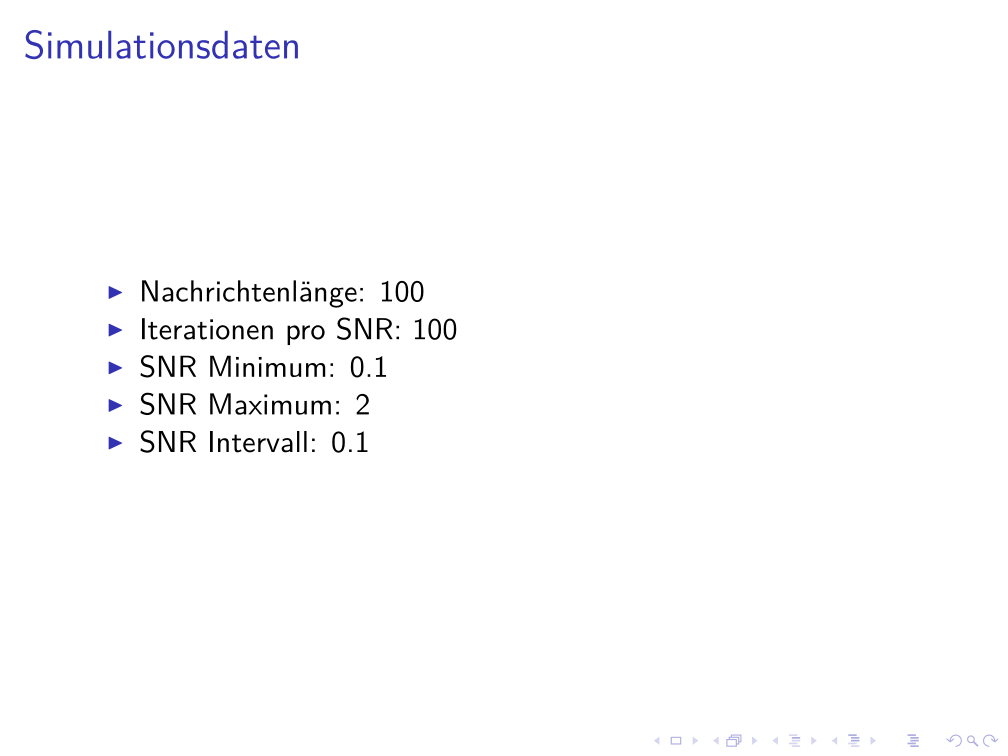
\includegraphics[width=\ScaleIfNeeded]{pictures/SimulationTurbo1} }
	\caption{Folie der Simulationsparameter}
	\label{pic:TurboSimulationParameter}
	\end{subfigure}
	\qquad
	\begin{subfigure}{0.45\textwidth}
	\centering
	\fbox{ 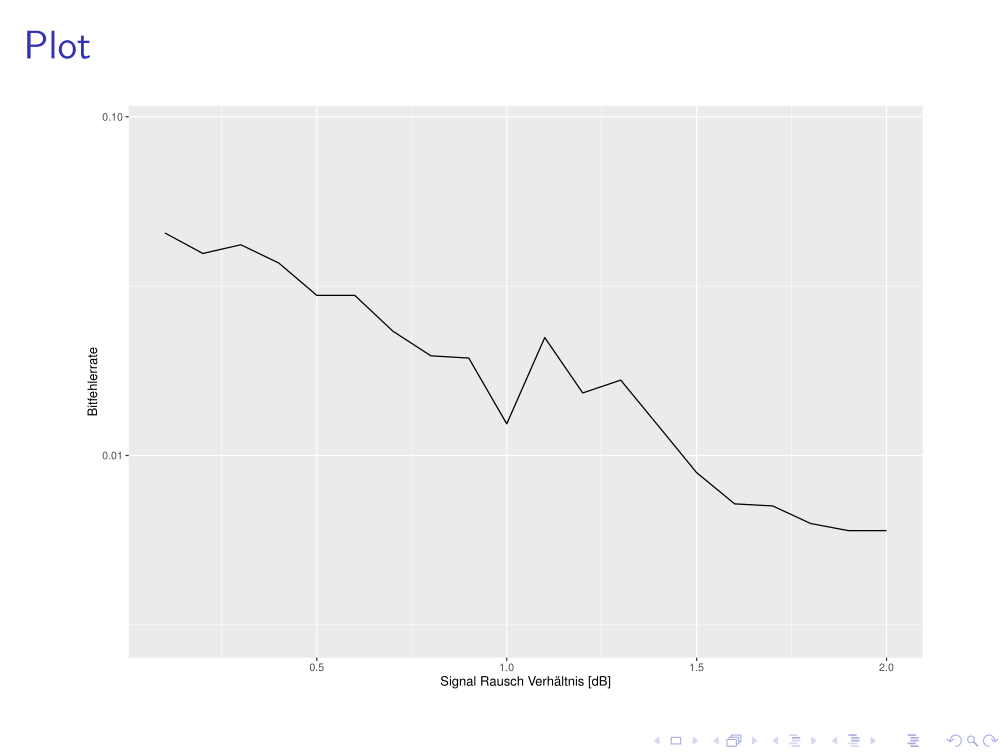
\includegraphics[width=\ScaleIfNeeded]{pictures/SimulationTurbo2} }
	\caption{Folie mit der Simulationsgrafik}
	\label{pic:TurboSimulationPlot}
	\end{subfigure}
\caption{Folien der Turbo-Kode Simulation}
\end{figure}

In Abbildung~\ref{pic:TurboSimulationParameter} sind die Nachrichtenlänge mit der getestet wurde und die Anzahl der Iterationen pro Signal/Rausch-Verhältnis zu sehen. Darunter sind noch die Ober- und Untergrenzen des Signal/Rausch-Verhältnisses dargestellt und die Schrittweite mit denen simuliert wurde.

Auf der nächsten Folie ist dann eine Grafik dargestellt, die in Abbildung~\ref{pic:TurboSimulationPlot} zu sehen ist. Dabei ist auf der x-Achse das Signal-Rausch-Verhältnis aufgetragen und auf der y-Achse wird die Bitfehlerrate dargestellt. Dabei sieht man sehr gut, dass mit größer werdenden Verrauschungsgrad die Bitfehlerrate steigt.

\FloatBarrier
\subsection{Kanalkodierung}
\label{sec:visualization_simulations_channelcoding}
Damit Block-, Faltungs- und Turbo-Kodes miteinander verglichen werden können, wird die Simulation mit den gleichen Parametern auf alle drei Kodierungsvarianten ausgeführt. Dadurch erhält man ein Ergebnis, das die Leistungsmöglichkeiten der drei Kodes sehr schön darstellt.

\begin{figure}[th]
\centering
\fbox{ 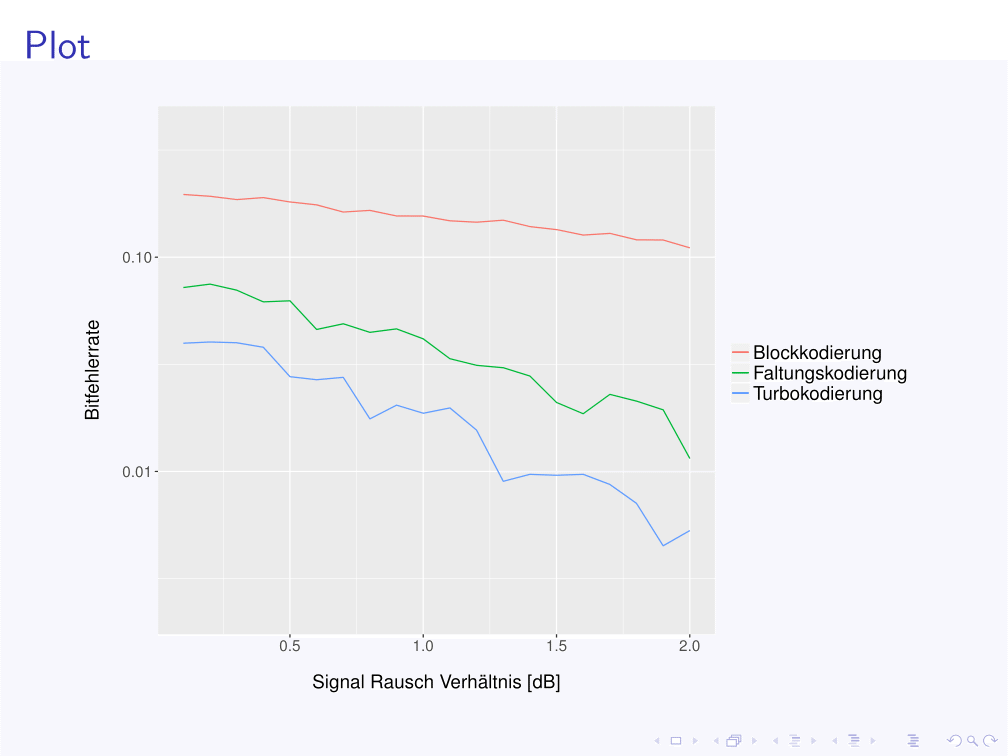
\includegraphics[width=\ScaleIfNeeded]{pictures/ChannelcodingSimulation1} }
\caption{Folie zum Vergleich der drei Kanalkodierungsvarianten}
\label{pic:ChannelcodingSimulation}
\end{figure}

In der Abbildung~\ref{pic:ChannelcodingSimulation} werden alle drei Ergebnisse der Simulation miteinander dargestellt. In der Legende sind die Farben der jeweiligen Kodes nachzusehen. Bei diesem Beispiel ist zu erkennen, dass wie erwartet der Blockkode das schlechteste Ergebnis liefert und der Turbo-Kode die geringste Bitfehlerrate aufweist. In der Mitte liegt erwartungsgemäß der Faltungskode.

\begin{figure}[th]
\centering
\fbox{ 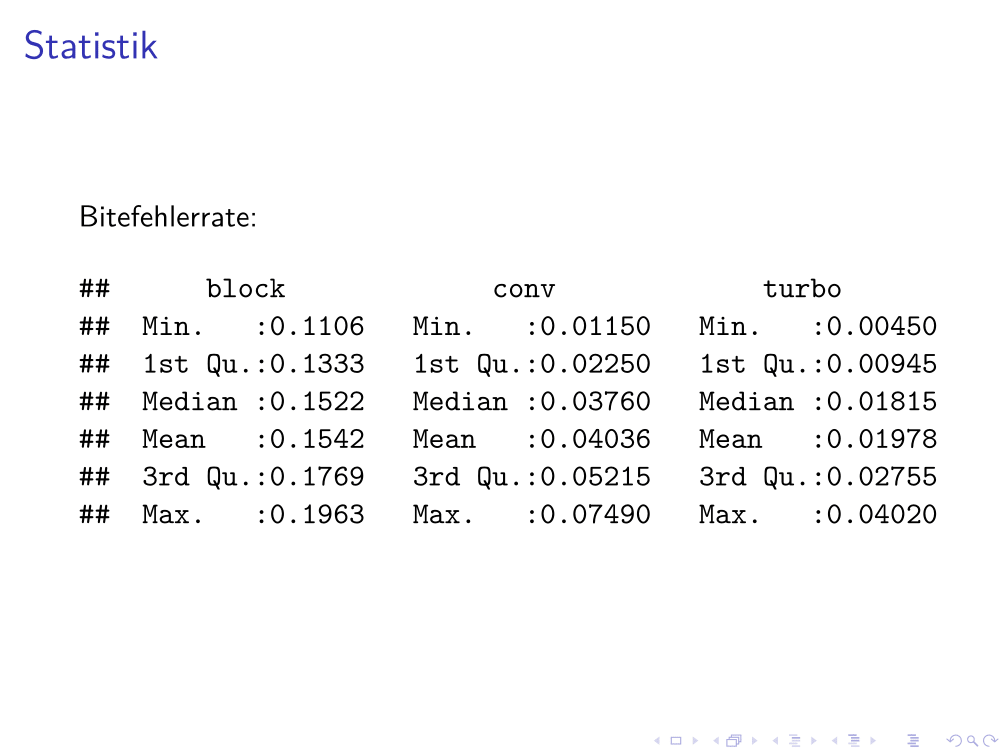
\includegraphics[width=\ScaleIfNeeded]{pictures/ChannelcodingSimulation2} }
\caption{Folie zur Darstellung der statistische Werte}
\label{pic:ChannelcodingSimulationStatistic}
\end{figure}

Auf der letzten Folie des Visualisierungsberichtes sind die statistischen Werte des jeweiligen Kodes angeführt. Daraus lassen sich auf den ersten Blick die maximale und minimale Bitfehlerrate des gewünschten Kodes herauslesen. Mit dem Durchschnittswert kann ein ganz einfacher Vergleich stattfinden, ohne jeden einzelnen Wert der Simulation zu vergleichen.

\FloatBarrier